\section{Methods}
In this chapter we will give insight into the software development method and our testing strategy. 

\subsection{Scrum}
We are going to work based off the scrum framework. Because we do not have a product owner and no real stakeholders we only use the things we think are good for our work method. This means we will have a daily meeting every moring we work on the project. Below we have listed the decisions we have made for our first sprint, this can be altered later so it is open for improvement, but this will be the skeleton for how we will do scrum during the project.
How we will do scrum:
\begin{itemize}
  \item Sprints of two weeks (Consists of eight working days at Windesheim).
  \item Daily scrum every workingday at 10:00.
  \item Sprint planning at the start of the sprint.
  \item Discuss sprint results with the team at the end of each sprint.
  \item Short retrospective at the end of each sprint.
  \item Scrummaster role will be filled in by Mark.
  \item Role of product owner will be filled in by the complete team.
\end{itemize}

\subsection{Test strategy}
We are going to test our user stories in different stages. First the producer of the code will test his own work before making a pull request. The producer will test if his own work meets the acceptance criteria and if the other user stories still work. After that, he will merge his branch with the development branch and solve any conflicts. After that the producer will test the code again. If it works it's ready for a pull request. When a pull request is made, the producer of the code will add new test cases to the test report. The reviewer will checkout the code and test it. Also, the reviewer will add results to the test cases in the test report that were added for that particular pull request.

~\\

We will make unit tests for the implemented user stories if we think it is testable, useful and necessary. We will use the Google Test C++ testing framework to write our unit tests.

\subsection{Tooling}
A lot of tooling is available for use in software development. We have chosen a set of tooling that we would like to use for this project. In this section we will explain the selection of tooling.

\paragraph{Telegram}
~\\ The chat application Telegram will be used to communicate with the group (or specific members of the group). A group chat will be created so that messages can be quickly shared with the group.

\paragraph{GitHub}
~\\ Git will be used as the source control system. All code (and documents) will be put inside a GitHub repository. Branches will be made for all changes and reviews will be done when a Pull Request is opened.

GitHub has a relatively new feature called "projects". A GitHub project consists of columns containing GitHub issues. This looks very similar to a tool called Trello. An example can be seen in \cref{fig:githubproject}. Since we will use GitHub quite extensively, we will use a GitHub project as our product backlog.

\begin{figure}
    \centering
    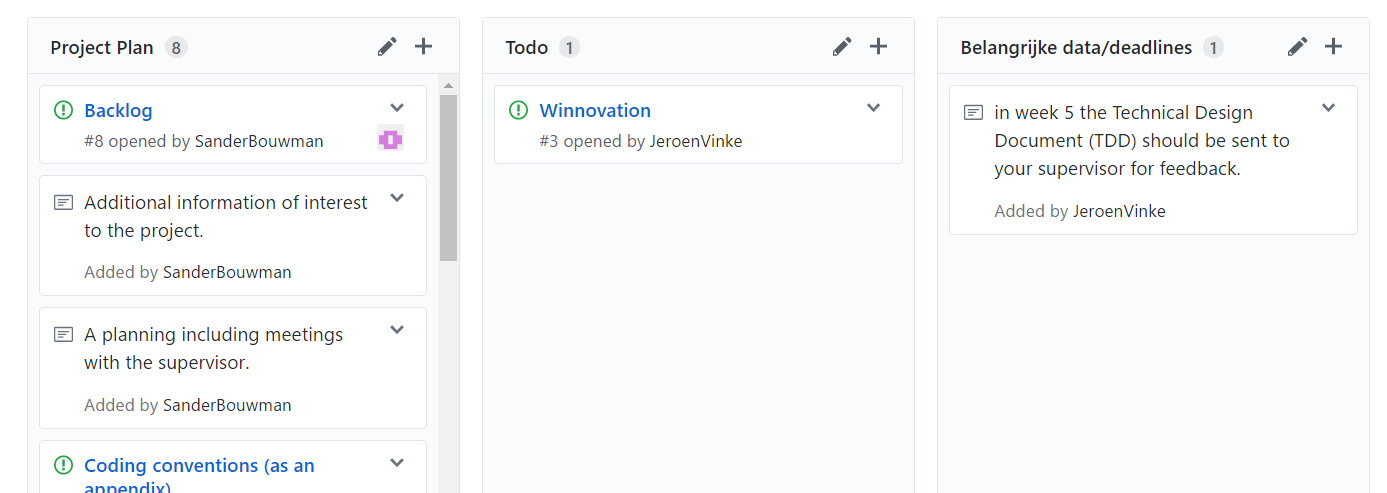
\includegraphics[scale=0.75]{images/github-projects.PNG}
    \caption{GitHub project}\label{fig:githubproject}
\end{figure}

\paragraph{Editors}
~\\ The group will use either Visual Studio or the Clion editor (depending on personal preference). 

\paragraph{TravisCI}
~\\ Since all our code is in a public GitHub repository, we can easily configure a build service using TravisCI. This build server will compile the game, run the linter and the unit tests. This will probably make the review process quicker.

